\documentclass[../structure.tex]{subfiles}
%\usepackage{../mypkg}
\begin{document}
\chapter{Methods and Implementation}
\hspace{2em}Before we discuss the ICP method and its implementation, let us first briefly review the linear algebra of affine transformations. If we have a point $[x,y,1]$ in homogeneous coordinate in 2D euclidean space and we want to move this point three units through the \textit{X axis}, $[x,y,1]^T a = [x+3,y,1]^T$, where $a$ will be  denoted as the affine matrix.

\begin{equation*}
\begin{bmatrix}
x \\ y \\ 1
\end{bmatrix}
\begin{bmatrix}
1 & 0 & 3 \\
0 & 1 & 0 \\
0 & 0 & 1
\end{bmatrix}
=
\begin{bmatrix}
x + 3 \\ y \\ 1
\end{bmatrix}
\end{equation*}

The example mentioned above is only for translation; we still have some other transformations (i.e. sheer, rotation and scale) which can be performed, as demonstrated in Figure \ref{fig:affine} for 2D shape.

\begin{figure}[h!]
\centering
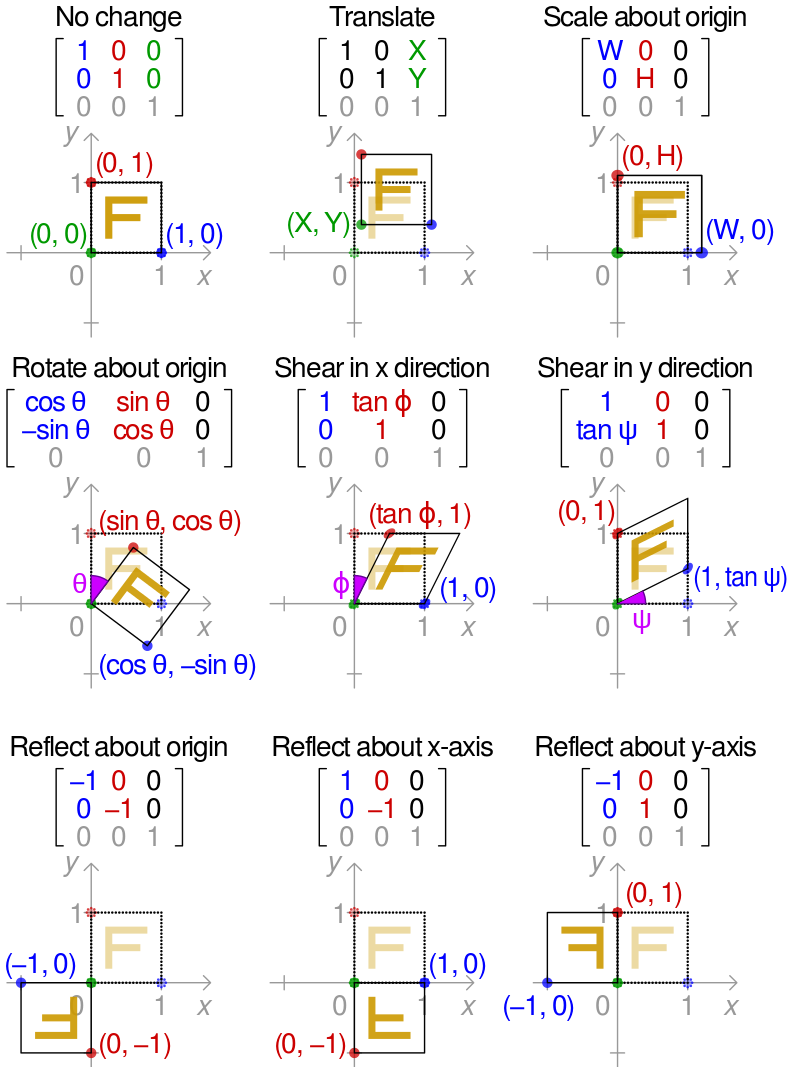
\includegraphics[scale=0.7]{007_affine}
\captionsetup{justification=centering}
\caption{2D affine transformation matrices.\\ Figure taken from en.wikipedia.org}
\label{fig:affine}
\end{figure}

We have shown how a 2D transformation occurs; the same principles apply to 3D as well, as demonstrated below:

\begin{equation*}
\begin{bmatrix}
\hat{x} \\ \hat{y} \\ \hat{z} \\ 1
\end{bmatrix}
\begin{bmatrix}
a & b & c & e\\
f & g & h & i\\
j & k & l & m\\
0 & 0 & 0 & 1
\end{bmatrix}
=
\begin{bmatrix}
x \\ y \\ z \\ 1
\end{bmatrix}
\end{equation*}

However,  this is still in the case of one point; if we have more points, as in our case, the equation above becomes:

\begin{equation*}
\begin{bmatrix}
\hat{x_{1}} & \hat{x_{2}} & \dots & \hat{x_{n}}\\
\hat{y_{1}} & \hat{y_{2}} & \dots & \hat{y_{n}}\\
\hat{z_{1}} & \hat{z_{2}} & \dots & \hat{z_{n}}\\
1 & 1 & \dots & 1
\end{bmatrix}
\begin{bmatrix}
a & b & c & e\\
f & g & h & i\\
j & k & l & m\\
0 & 0 & 0 & 1
\end{bmatrix}
=
\begin{bmatrix}
x_{1} & x_{2} & \dots & x_{n}\\
y_{1} & y_{2} & \dots & y_{n}\\
z_{1} & z_{2} & \dots & z_{n}\\
1 & 1 & \dots & 1
\end{bmatrix}
\end{equation*}

\pagebreak

\hspace{2em}As we are implementing the registration method, we are going to consider two objects, target graph $T$, which remains fixed, and template graph $S$, which moves iteratively until it reaches the optimal alignment with target graph $T$. To do so, we use Iterative Closest Point (ICP) as previously discussed (see Figure \ref{fig:icp}). With ICP, for each point on the template graph $S$, we look for the closest point on the target graph $S$. Then we start moving each point in $S$ to a correspondent point in $T$ with respect to stiffness. After solving the cost function by using \textit{LSQR} iteratively until the distance between the last iteration and the current iteration is less than a parameter selected by the user, we have a separate \textit{Affine Transformation Matrix} ($X = [X_{1}, X_{2}, X_{3}, ...,X_{n}]$) for each point in the template graph $S$ that moves separately whilst keeping the original neighbors as close to each other as possible. This type of registration is called non-rigid registration.

\begin{figure}[h!]
\centering
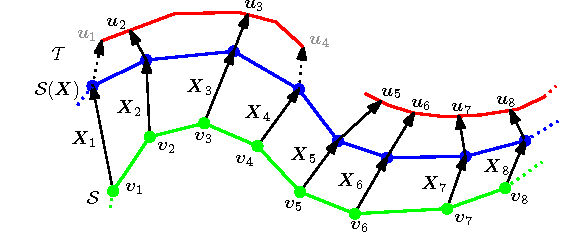
\includegraphics[scale=0.5]{001_conn}
\captionsetup{justification=centering}
\caption{The template graph $S$ (green) moves toward target graph $T$ (red) and become graph $S(X)$ by applying local deformation. Each point $v_{i}$ in the template graph $S$ moves toward correspondence point $u_{i}$ in the target graph $T$ by applying local affine matrix $x_{i}$. Some points does not have correspondent point, but they still move because of stiffness \cite{Amberg2007}.} 
\label{fig:icp}
\end{figure}

We implement the method in \cite{Amberg2007} by using the Python programming language, Spyder as an IDE \cite{spyder} and several packages, namely PlyFile \cite{plyfile}, DIPY \cite{nipy}, NiBabel \cite{nipy}, Open3D \cite{Zhou2018}, Numpy \cite{numpy}, Scipy \cite{scipy}, Scikit-learn \cite{sklearn} and Matplotlib \cite{matplotlib}.

\section{Data preparation}
\hspace{2em}In this work, we follow the method in \cite{Amberg2007} which is implemented for surface graphs. However, due to differences between data used in \cite{Amberg2007} which are surface graphs saved in either points cloud or mesh format, and our data which are pathways in streamlines format and saved in \textit{ply} file as shown in Figure \ref{fig:data}, we had to build a tool for reading the \textit{ply} file format as streamlines and build graphs out of it. In this case, each \textit{ply} file has one pathway.

\subsection{The PLY file}
\hspace{2em}Let us illustrate a bit of our data and the \textit{ply} files we used to save our data, as shown in Figure \ref{fig:data}. The \textit{ply} file consists of two parts: the header and body. The header consists of all information that is necessary to parse the file, and the body has the data itself.

\begin{figure}[h!]
\centering
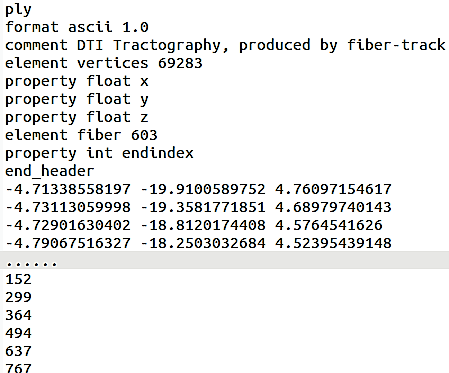
\includegraphics[scale=1]{002_data}
\captionsetup{justification=centering}
\caption{A sample of a brain pathway saved in a \textit{ply} file.}
\label{fig:data}
\end{figure}

\begin{itemize}
\item The first line represents the file type
\item The second line is the file format
\item The third line is a comment
\item The fourth line contains the name and corresponding number of the first group of elements (each ply file can have any number of elements). Specifically, we can see that there are 69283 vertices in the file.
\item The 5th, 6th and 7th lines shows that the first group of elements has three properties, each of them in float format as well as  the name of each property.
\item The 8th line shows the second group of elements which has 603 fiber tracts.
\item The 10th line shows the end of the header part.
\item The remaining lines are the body of the file which has all the data, with each element in one line.
\end{itemize}

\hspace{2em}Before we start registering the graphs, it is better to have the initial position which makes the template graph $S$ as close as possible to the target graph $T$ and in the best possible alignment before ICP. To do so, we use Principal Components Analysis as illustrated below.

\section{Principal Components Analysis }
\hspace{2em}Before applying PCA, we scale the template graph $S$ and the target graph $T$ to $[0,1]$. This is done by subtracting all points from the minimum value in the graph and then dividing them by the maximum value in the graph. Next, we apply PCA and use $[-1,1]^3$ cube combination and measure the Euclidean distance between each point in the template graph to the closest point in the target graph as illustrated in the equation $\sum ||v_i-v_j||_F^2$ where $v_i \in S, v_j \in T$. This formula is applied eight times to select the combination with the minimum distance as illustrated in Table \ref{table:cube} and in Figure \ref{fig:pca}. Because we have to keep the target graph $T$ fixed, we apply the transformation calculated from both graphs on template graph $T$, thus the transformation of target graph $T$ has to apply oppositely.
\vspace{2em}
\begin{center}
\begin{table}[h]
	\begin{tabular}{| c | c | c | c | c | c | c | c |}
	\hline
	1 & 2 & 3 & 4 & 5 & 6 & 7 & 8\\
	\hline
	(x,y,z) & (x,y,-z) & (x,-y,z) & (x,-y,-z) & (-x,-y,z) & (-x,y,-z) & (-x,y,z) & (-x,-y,-z)\\
	\hline
	\end{tabular}
\caption{$[-1,1]^3$ cube combination}
\label{table:cube}
\end{table}
\end{center}

\begin{figure}[h!]
	\centering
	\begin{subfigure}[b]{0.59\textwidth}
	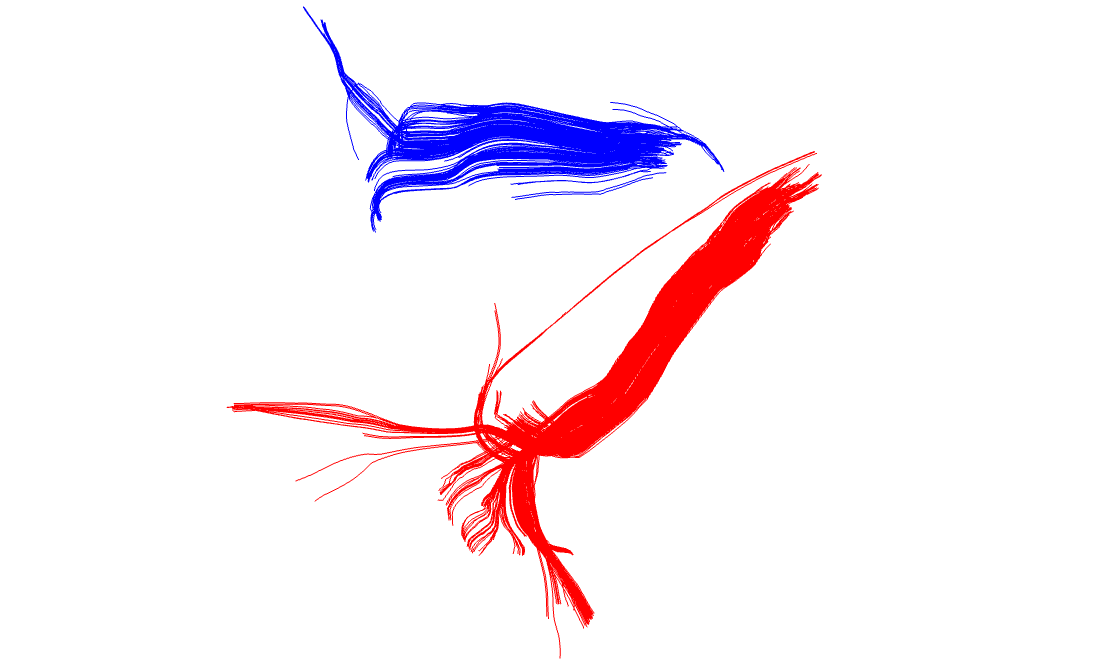
\includegraphics[width=\textwidth]{003_original}
	\caption{Original position}
	\end{subfigure}
	% separate
	\begin{subfigure}[b]{0.40\textwidth}
	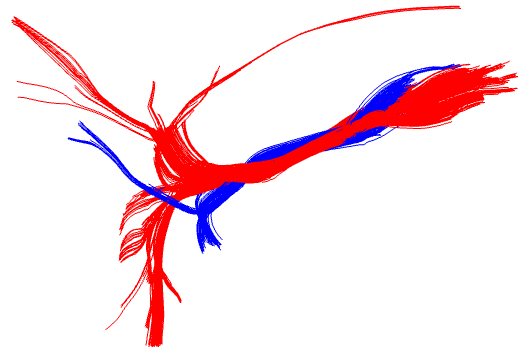
\includegraphics[width=\textwidth]{004_pca}
	\caption{After PCA}
	\end{subfigure}
\caption{Applying PCA for initial alignment before ICP}
\label{fig:pca}
\end{figure}

%\pagebreak

%\vspace{2em}
\section{The Cost Function}
\hspace{2em}The simplest form of the cost function is shown in the equation (\ref{equ:equation1}):

\begin{equation}
\label{equ:equation1}
cost(Ax,b) = ||Ax-b||^2
\end{equation}

Where $A$ and $b$ are complexes of matrices including template graph and target graph respectively as we will illustrate below

This simple form of the cost function makes it easy to solve by the \textit{LSQR} (\textit{scipy.sparse.linalg.lsqr}) algorithm which is the implementation of a conjugate-gradient type method for solving sparse linear equations and sparse least-squares problems \cite{Paige1982a}.

To illustrate the cost function more we need to divide it into three parts, as shown in equation (\ref{equ:costFun1}). These include the distance term $E_{d}$, stiffness term $E_{s}$, and landmark term $E_{t}$.

\begin{equation}
E(X) = E_{d}(X) + \alpha E_{s}(X) + \beta E_{t}(X)
\label{equ:costFun1}
\end{equation}

\subsection{Distance Term}
\hspace{2em}The first part of the cost function (\ref{equ:costFun1}) is the distance term, it represent the summation of distances between each point in the template graph $S$ and its correspondent point in the target graph $T$, To simplify the equation, we will consider the distance between one point in the template graph $S$ and its correspondent point in the target graph $T$ as illustrated in equation (\ref{equ:distance2}):

\begin{equation}
dist^2(T,X_{i}v_{i}) = ||X_{i}v_{i}-u_{i}||^2
\label{equ:distance2}
\end{equation}

where $T$ is the target graph, $X_{i}$ is the correspondent affine matrix in size $3\times4$, $v_{i}\in V$ is template graph $S$ vertex in homogeneous coordinates $v_{i} = [x,y,z,1]$ because we want to include transformation on affine matrix $X_{i}$.

To get overall distance we calculate it using equation (\ref{equ:distance1})

\begin{equation}
E_{d}(X) = \sum_{v_{i} \in V} w_{i}dist^2(T,X_{i}v_{i})
\label{equ:distance1}
\end{equation}

where $W = [w_{1}, w_{2}, w_{3}, ..., w_{n}];\quad w_{i}\in [0,1]$ is weight which is \textit{one} if the correspondent point distance is below the threshold and \textit{zero} if not, even some points in template graph do not have correspondences in target graphs $T$, they move with their neighbors due to stiffness term. 

We calculate the result of $||X_{i}v_{i}-u_{i}||^2$ while the algorithm reduces the distance and improves the alignment iteratively.

If we look back to equation (\ref{equ:distance1}) and combine it with equation (\ref{equ:distance2}), then we have a complete equation (\ref{equ:distance3})

\begin{equation}
\bar{E}_{d}(X) = \sum_{v_{i}\in V} w_{i}||X_{i}v_{i}-u_{i}||^2
\label{equ:distance3}
\end{equation}
\begin{equation*}
= \left\|(W \otimes I_{3}) \left(
\begin{bmatrix}
X_{1} & & \\
& \ddots & \\
& & X_{n}
\end{bmatrix}
\begin{bmatrix}
v_{1} \\ \vdots \\ v_{n}
\end{bmatrix} -
\begin{bmatrix}
u_{1}\\ \vdots \\ u_{n}
\end{bmatrix}
\right) \right\|^2
\end{equation*}\\

where $W = diag(w_{1},\dots, w_{n})$ corresponds to the weights in the diagonal matrix multiplied by the Kronecker product $\otimes$ to $I_{3}$ identity matrix. $X$ is a diagonal matrix of $X_{i}$ that we need to solve and is multiplied by vertices matrix $V=[v_{1},v_{2},v_{3}, \dots,v_{n}]^T$ of template graph $S$, subtracted by the corresponding vertices matrix $U=[u_{1},u_{2},u_{3}, \dots,u_{n}]$ of the target graph $T$.

Let us clarify how \textbf{Kronecker product} works, it is operation of two matrices of arbitrary size denoted by $\otimes$. It is a generalization of the outer product, (denoted by the same symbol) from vectors to matrices, and gives the matrix of the tensor product with respect to a standard choice of basis.

For instance, If $A$ is an $m \times n$ matrix and $B$ is a $p \times q$ matrix, then the Kronecker product $A \otimes B$ is the $mp \times nq$ block matrix:

\begin{equation*}
A \otimes B =
\begin{bmatrix}
a_{11}B & \dots  & a_{1n}B \\
\vdots  & \ddots & \vdots  \\
a_{m1}B & \dots  & a_{mn}B
\end{bmatrix}
\end{equation*}\\

Thus, the result of $W \otimes I_{3}$ is a $3n\times 3n$ matrix, where matrix $X$ has size $3n\times4n$, $V$ has a shape $4n\times1$ and $U$ has shape $3n\times1$.

We continue to reform the equation to be easily differentiated and implemented by converting it into canonical form. First we swap the positions of the $X$ and $V$ matrices, then we define a sparse matrix $D$ which contains the vertices $v_{i} \in V$ in diagonal position as demonstrated below:

\begin{equation}
D =
\begin{bmatrix}
v_{1}^T & & & \\
& v_{2}^T & & \\
& & \ddots & \\
& & & v_{n}^T
\end{bmatrix}
\label{equ:matD}
\end{equation}\\

The new format of the equation becomes:

\begin{equation}
\bar{E}_{d}(X) = ||W(DX-U)||_{F}^2
\label{equ:distance4}
\end{equation}

\hspace{2em}Where the matrix $W$ has size $n\times n$, the matrix $D$ has size $n\times 4n$ (vertices $v_{i}$ are in homogeneous coordinates $[x,y,z,1]^T$), $X$ has size $4n\times 3$, $U$ does not change with shape $n\times 3$ (vertices $u_{i}$ are in 3D coordinate) and $||.||_{F}$ denote the Frobenius norm.

\subsection{Stiffness Term}
\hspace{2em}The stiffness term is the second part of the equation (\ref{equ:costFun1}). It regularizes the deformation of template graph $S$ by penalizing the weighted difference of the transformations of neighboring vertices under the Frobenius norm $||.||_{F}$ using a weight matrix $G := diag(1, 1, 1, \gamma)$ \cite{Amberg2007}, that keeps the distance between vertices which are neighbours (i.e., vertices which have an edge between them) and also in the same tract constant.
\begin{equation}
E_{s}(X) = \sum_{i,j \in E} ||(X_{i} - X_{j})G||_{F}^2
\label{equ:stiffness1}
\end{equation}

The parameter $\gamma$ is used to balance the rotation and skew against translation while transforming the template graph $S$ \cite{Amberg2007}. In our case $\gamma$ is \textit{one} as we have already scaled our data into the $[-1, 1]^3$ cube.

To make our function solvable directly we need to write it as a quadratic function. Therefore we use twelve parameters per vertex in $3 \times 4$ shape and an $\alpha$ parameter in equation (\ref{equ:costFun1}) which is a constant that manages the contribution of the stiffness term; when it is high, the neighbor vertices do not move far away from each other and when it is low, a greater deformation can occur.
The part $||.||_{F}$ is the \textit{Frobenius norm} which is illustrated in the example below \cite{Amberg2007}:

\begin{equation*}
||A||_{F} = \sqrt{\sum_{i=1}^m \sum_{j=1}^n |a_{ij}|^2}
\end{equation*}

To make the stiffness term more simpler and applicable, we put it in the form below:

\begin{equation}
E_{s}(X) = ||(M\otimes G)X||_{F}^2
\end{equation}

where $M$ is a node-arc incidence matrix defined for directed graphs. The number of rows in this matrix equal the number of nodes (vertices) and the number of columns equal the number of arcs (edges) on the graph and the values must be \textit{zeros, ones and/or minus ones}. The value will be \textit{zero} if the edge on this column is not connected to the vertex on this row where the value lies, otherwise, the value must be either $1$ or $-1$; it will be $1$ if the edge direction is coming towards the vertex and $-1$ otherwise. As illustrated in the Figure \ref{fig:directed_graph}, the matrix $M$ has size $e\times n$ where \textit{e} and \textit{n} are the number of edges and vertices respectively. $G = diag(1,1,1,\lambda)$ is the diagonal matrix and the result of $M \otimes G$ is $4e \times 4n$ matrix.


\begin{figure}[h!]
\centering
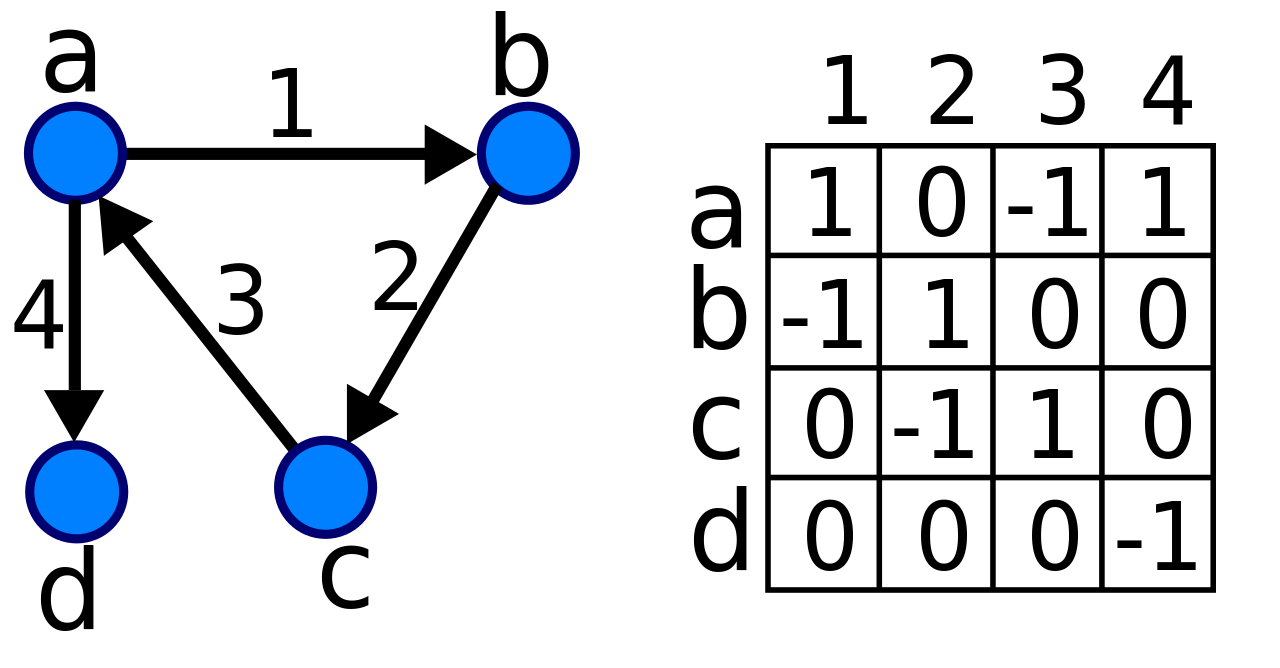
\includegraphics[scale=0.2]{006_direct_graph}
\captionsetup{justification=centering}
\caption{Oriented graph with corresponding incidence matrix.\\ Figure taken from en.wikipedia.org}
\label{fig:directed_graph}
\end{figure}
\pagebreak
\subsection{The Landmark Term}
\hspace{2em}The landmark term gives the initial position of the template graph $S$ shown in equation (\ref{equ:landmark1}) below:

\begin{equation}
E_{l}(X) = \sum_{(vi,l) \in L}||(X_{i}v_{i} - l)||^2
\label{equ:landmark1}
\end{equation}\\

Where $L = \left\{(v_{i1},l_{1}),(v_{i2},l_{2}),...,(v_{il},l_{l})\right\}$ is the set of landmarks that maps the template graph $S$ to the target graph $T$. The $\beta$ parameter in equation (\ref{equ:costFun1}) controls the influence of the landmark term.

\subsection{The Final Cost Function}
After simplifying each term separately, we are going to join them together in one equation, (\ref{equ:costFun2}) as outlined below:

\begin{equation}
\bar{E}(X) = \left\|
\begin{bmatrix}
\alpha M \otimes G \\ WD \\ \beta D_{L}
\end{bmatrix}
X -
\begin{bmatrix}
0 \\ WU \\ U_{L}
\end{bmatrix}
\right\| ^2
\label{equ:costFun2}
\end{equation}\\

The current form of the function can be minimized by setting its derivative to zero and solving it as a linear equation. The minimum value of $\bar{E}(X)$ is when $X = (A^T A)^{-1} A^T B$.

Even $A$ a sparse matrix and most of its values are zeros, however, it is still a large matrix and requires the most time to solve the equation. In order to solve the equation at a faster speed, we omitted the landmark term because we already have the initial position by applying PCA. Once we omit the landmark term, the function will be:

\begin{equation}
E(X) = \left\|
\begin{bmatrix}
\alpha M \otimes G \\ WD
\end{bmatrix}
X -
\begin{bmatrix}
0 \\ WU
\end{bmatrix}
\right\| ^2
= ||Ax - b||_{F}^2
\label{equ:costFun3}
\end{equation}\\

\subsection{Implementing Cost Function}
\hspace{2em}To implement the equation (\ref{equ:costFun3}), we use sparse matrices to build most of the matrices, that because the majority of values in these matrices are zeros.

\begin{figure}[h!]
\centering
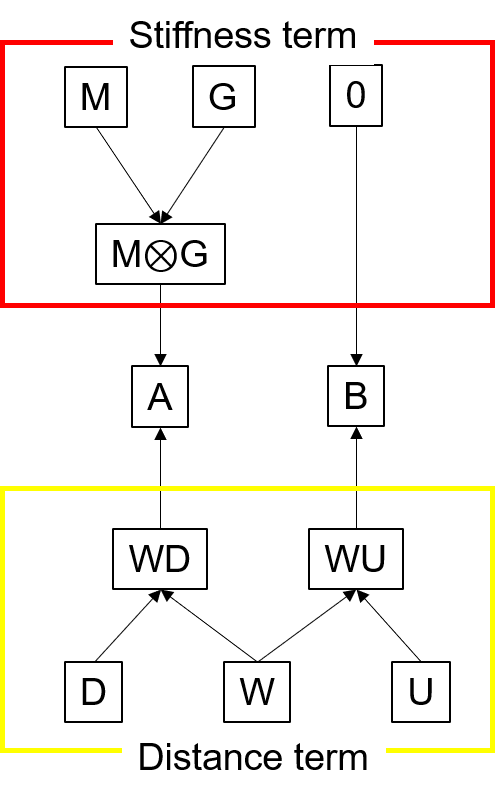
\includegraphics[scale=0.8]{010_cost_fun}
\captionsetup{justification=centering}
\caption{Building the cost function flow}
\label{fig:cost_flow}
\end{figure}

Figure \ref{fig:cost_flow} shows how we are going to implement the cost function. The first step is measuring the Euclidean distance between each point $v_{i}\in V$ in the template graph $S$ and its correspondent point $u_{i}\in U$ in the target graph $T$ using \textit{K-D Tree}, then we filter distances by a threshold value (which is a parameter whose criteria for selection will be discussed later ) to define \textit{zeros} and \textit{ones} and put them diagonally on $n\times n$ sparse matrix \textit{W}.

\begin{equation*}
W =
\begin{bmatrix}
w_{1}^T & & & \\
& w_{2}^T & & \\
& & \ddots & \\
& & & w_{n}^T
\end{bmatrix}
\end{equation*}\\

We continue building variables in equation (\ref{equ:costFun3}). Now we have the matrix \textit{W}, to calculate $W\times D$ we must build \textit{D}, which is $n\times 4n$ sparse matrix. To do so, we join all tracts on the template graph $S$ to have point cloud matrix $V=[v_{1}, v_{2}, v_{3}, \dots , v_{n}]^T$ which is a $n\times 3$ matrix and we add one more column at the end of the matrix to have homogeneous coordinates $v_{i}=[x,z,y,1]$. Then we take each vertex $v_{i} \in V$ and place it diagonally in the sparse matrix \textit{D}, as shown in equation (\ref{equ:matD}). Finally, to get $n\times 4n$ matrix \textit{WD}, we calculate the dot product of $W\times D$ as in equation (\ref{equ:costFun3}).

As we already have $n\times 3$ matrix $U=[u_{1}, u_{2}, u_{3}, \dots , u_{n}]$, which is point cloud of target graph $T$. And we have $W$ as calculated above, we can calculate $n\times 3$ matrix $WU=W\times U$ as $W$ dot product $U$.

The stiffness term is only for the template graph $S$ as we can see in equation (\ref{equ:costFun3}). To implement the stiffness term, we need to have $M$ and $D$. First, we build diagonal sparse matrix $G = diag(1,1,1,\lambda)$ and $\lambda=1$ in our case. Then we build an $e\times n$ node-arc matrix \textit{M}. To do so, we use the streamlines form template graph $S$ which has the connections of between points in the same tract (streamline). We next calculate Kronecker product of $M \otimes G$. The $\lambda$ parameter is a variable the user can adjust depending on the data.

To have the final form of the cost function, we vertically stack $\alpha M \otimes G$ on top of $WD$ in one sparse matrix $A$ with size $n\times 4n$.  The sparse matrix $A$ is a part of the equation (\ref{equ:costFun3})

As previously discussed, we already have \textit{WU}; To get the sparse matrix $b$ in the equation (\ref{equ:costFun3}), we create a sparse matrix of zeros with size $n\times 3$ and vertically stack it on top of \textit{WU}.

The cost function $||Ax-b||_{F}^2$ can then be solved by using \textit{LSQR}, which takes $A$ and $b$ as parameters and returns $X=[x_{1}, x_{2}, x_{3}, \dots, x_{n}]$. However, as we can observe, $b$ in our case is an $n\times 3$ matrix and \textit{LSQR} from \textit{SciPy} takes $b$ as vector only. To solve this problem, we use the fundamental principle of matrix multiplication by applying \textit{LSQR} for each column in matrix $b$.

To achieve the optimal alignment we calculate \textit{LSQR} iteratively until there is no more improvement in the registration or the improvement is minor.

When we have the optimal alignment, we need to have the original form of pathways as streamlines as discussed in beginning of this chapter. To do so, first, we need to get point cloud form $V$ of template graph $S$ by calculating the dot product of the $D\times x$. We get the matrix $x$ as the result of \textit{LSQR}. 

Finally, we can convert the point cloud of the template graph back to the original form of pathways as streamlines.

Finally for visualization, we customize functions from \textit{Open3D} \cite{Zhou2018} library to view brain fiber pathways.

\begin{figure}[h!]
\centering
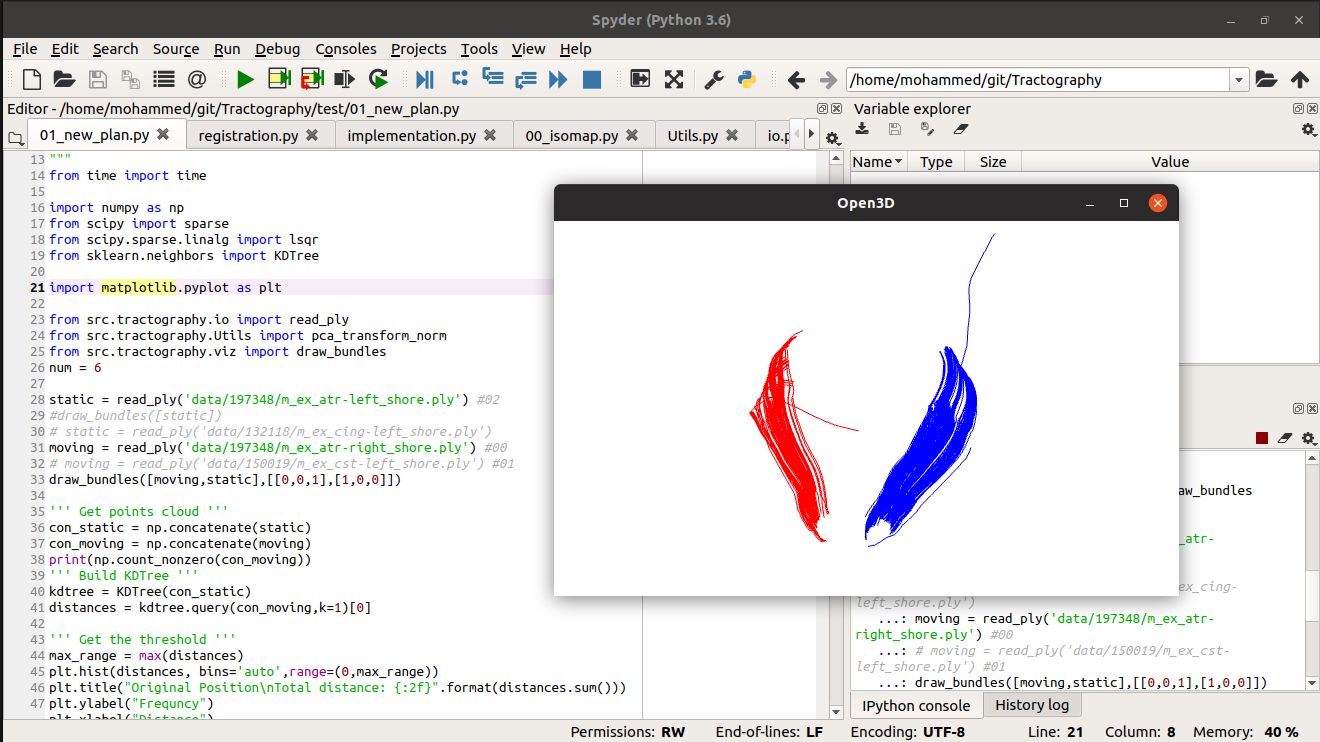
\includegraphics[scale=0.3]{008_ide}
\captionsetup{justification=centering}
\caption{Spyder IDE and Open3D visualization tool}
\end{figure}

\end{document}

